\documentclass{article}
\usepackage{graphicx} % Required for inserting images

\title{NRS SRAD Power Distribution Unit}
\author{Timonas Juonys, Herman Darjes }
\date{September 2024}

\begin{document}

\maketitle

\section{Introduction}
The Power Distribution Unit is the component responsible for supplying the avionics with power at the appropriate voltages, whilst logging the power draw. This is implemented as a printed circuit board. The functionality of the PDU is as seen in figure \ref{fig:pdu_overview}.

\begin{figure}
    \centering
    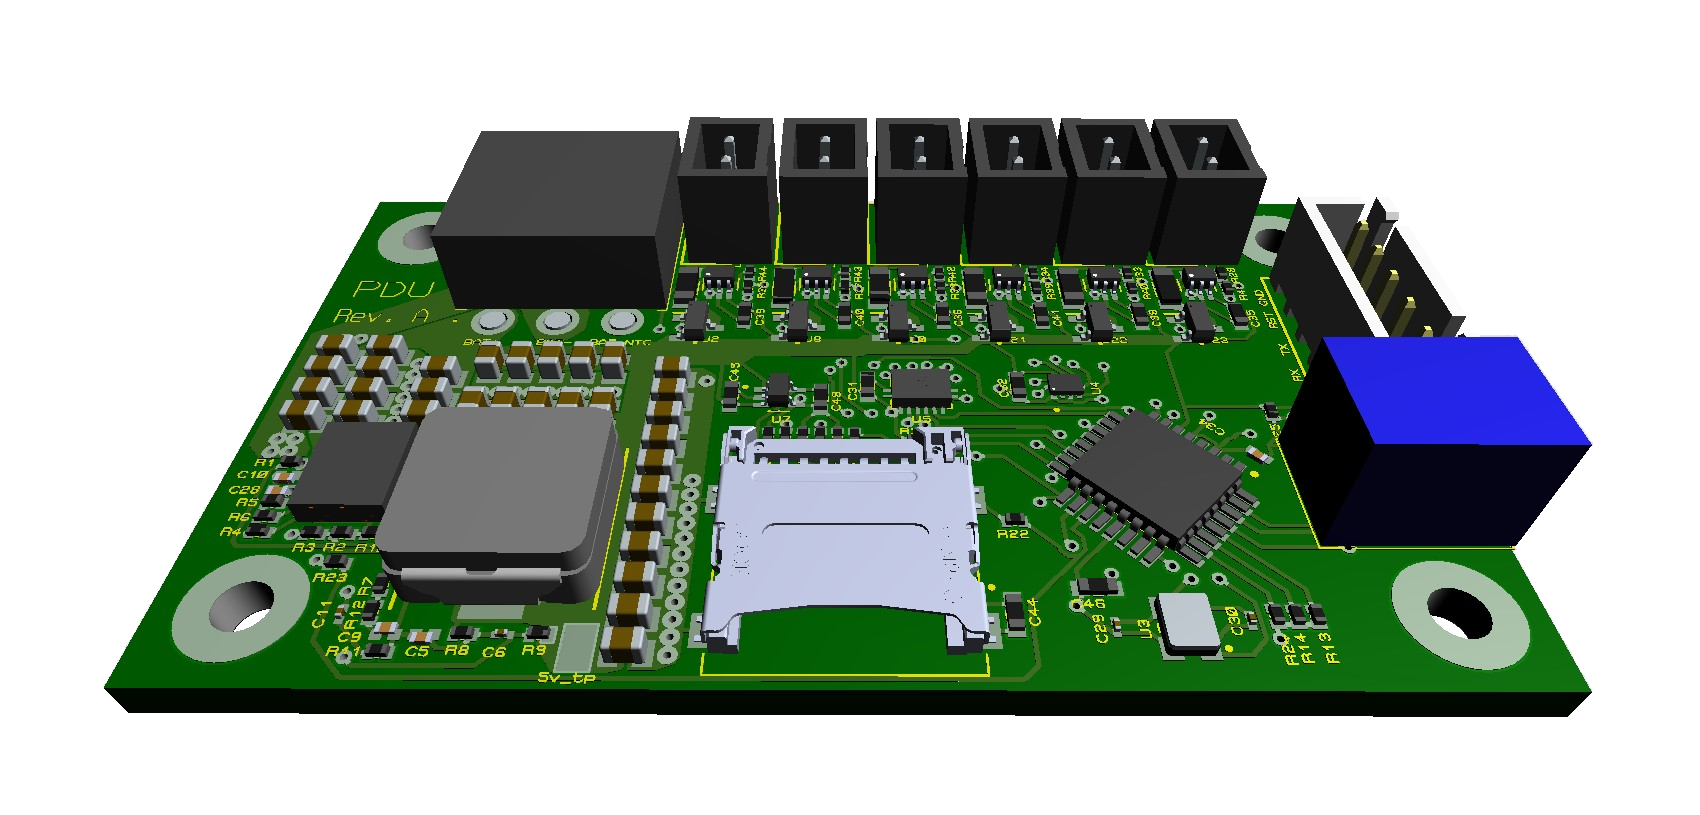
\includegraphics[width=1\linewidth]{img/NRS_PDU_PCB.png}
    \caption{Render of PCB with components}
    \label{fig:pdu_render}
\end{figure}

\begin{figure}
    \centering
    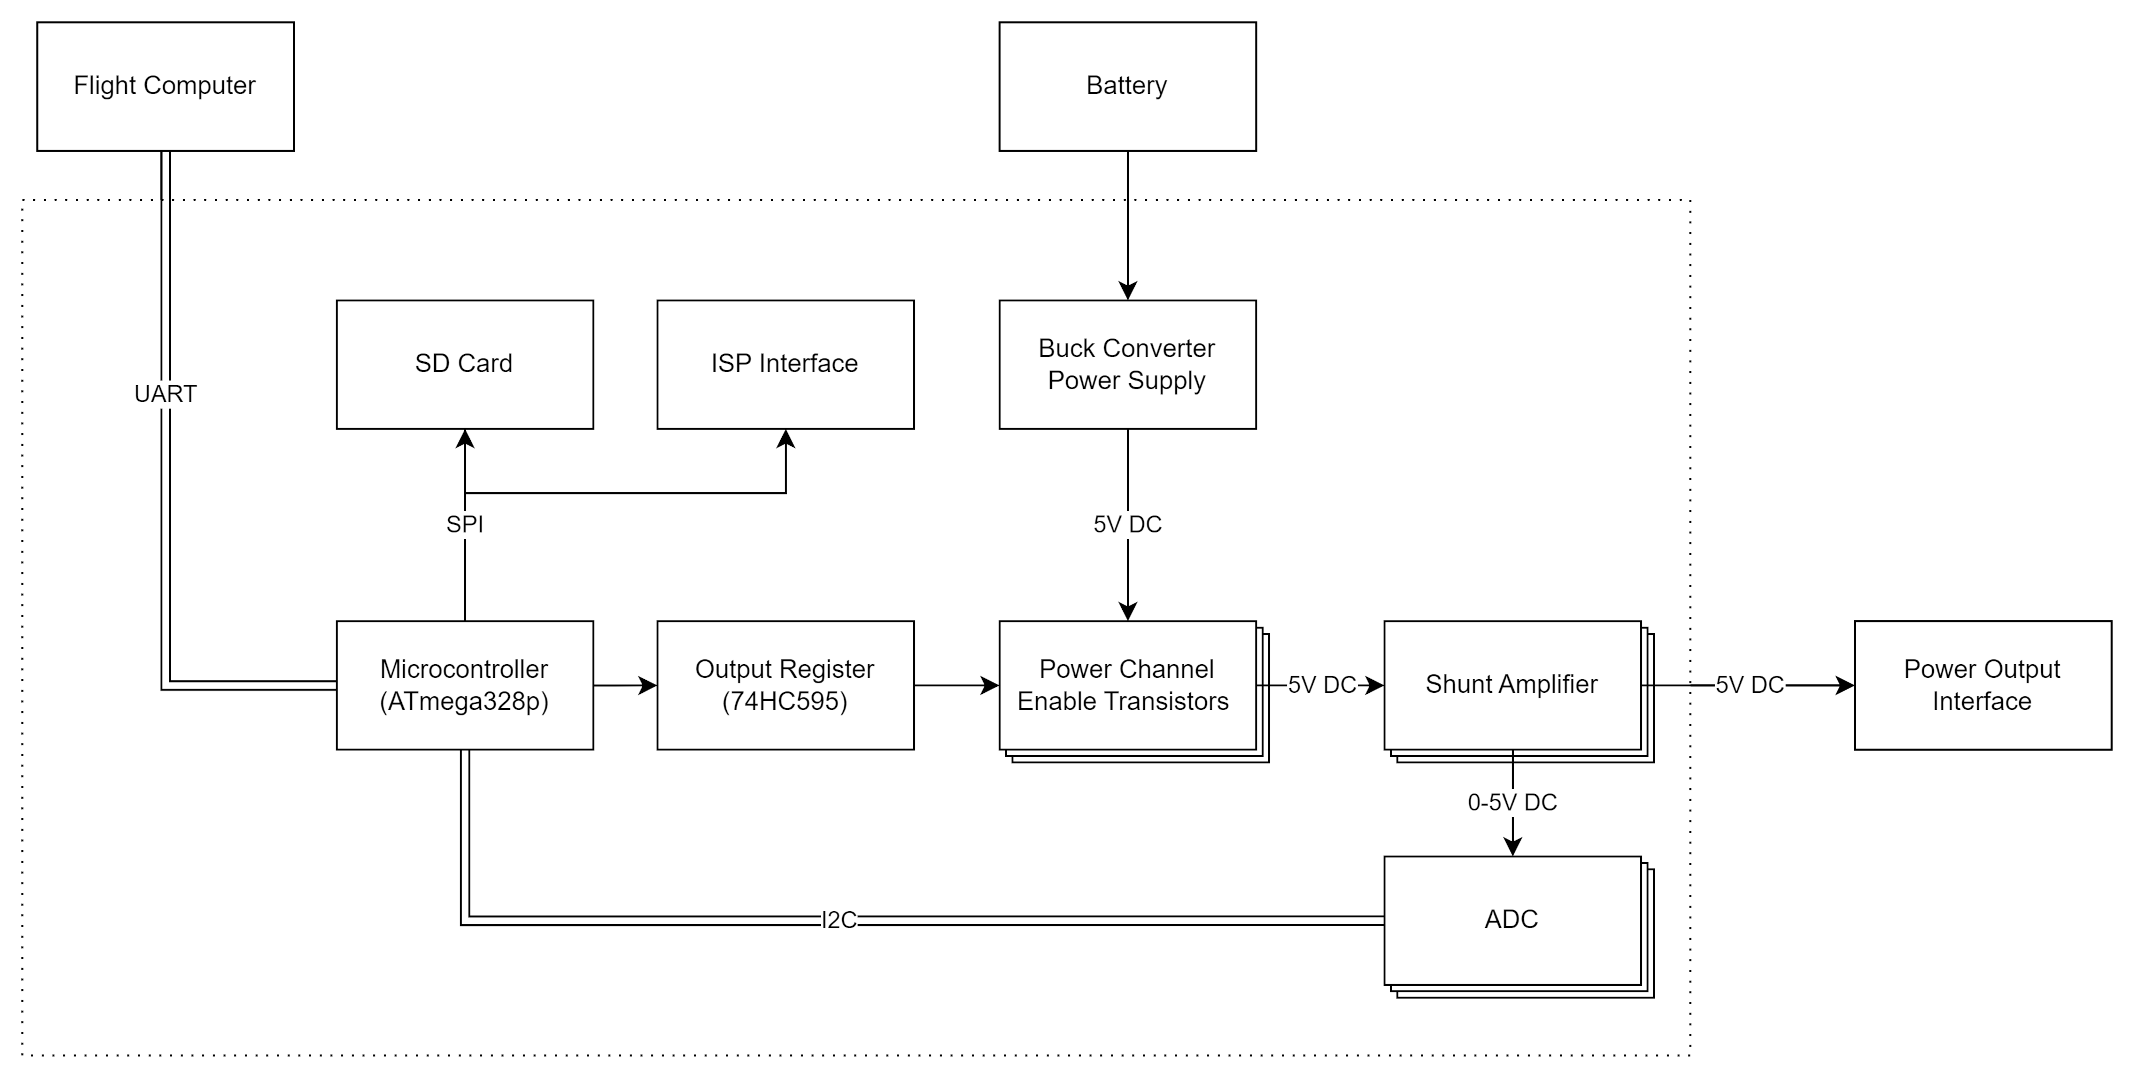
\includegraphics[width=1\linewidth]{img/pdu_overview.png}
    \caption{Overview of Power Distribution Unit}
    \label{fig:pdu_overview}
\end{figure}
\section{Requirements}
The PDU is required to have six individual, controllable, off-by-default electrical channels to supply three cameras, two servos and the flight computer with power, including an additional auxiliary channel. The system must be able to supply maximum power at the ambient temperature of 60°C-70°C. See table \ref{tab:pdu_pwr_config} for power and channel configuration and rating.
\\
In addition to power supply, the PDU must have logging functionality for currents, voltages and temperatures, this data will be saved to an SD-card.
\\
The PDU is controlled by the Flight Computer through the UART protocol to enable and disable logging and the individual channels.

\section{Power Channels}
Power channels will be enabled and disabled using transistors controlled by the microcontroller. All power channels have a high side shunt amplifier connected to ADC for current sensing.
\begin{table}
    \centering
    \begin{tabular}{|c|c|c|} \hline 
         \textbf{Quantity} &  \textbf{Current at 5V (max)}& \textbf{Description} \\ \hline 
 3& 2A&Camera\\ \hline 
 2& 3A&Servo\\ \hline 
 1& 1A&Flight Computer and PDU\\ \hline 
 1& 2A&Auxiliary\\ \hline 
 Total:& 15A&\\ \hline
    \end{tabular}
    \caption{Power channel configuration}
    \label{tab:pdu_pwr_config}
\end{table}

\section{Components}
\subsection{Buck IC}
The requirements called for 15A total at 5V, so we needed to design a buck converter capable of that. We chose to use a single buck converter contra several, since this way it would be more compact, and many IC's were available in this current range. TPS53353DQPR was chosen because it had generous specs of 20A continuous current, it could output 5v out, and it had some examples of usual implementations in its data sheet. 

\subsection{Microcontroller}
The microcontroller has to be compatible with the Arduino UNO, because of our familiarity with the platform, and the accessibility of software libraries. With this in mind, we chose the ATmega328P. To expand output pins, a SN74HC595 shift register is selected with easy implementation and simple functionality in mind. 
\\
In System Programming (ISP) is implemented through a header for burning the bootloader. To further program the microcontroller, an external FTDI converter is connected to the Flight Computer connector though a programming cable.

\subsection{Current Sensing}
For current sensing, the Texas Instruments INA214 Current Sense Amplifier was implemented with shunt resistors. We chose to sense current on the high side contra the low side, so that the ground was the same for all devices in the system. This required a differential amplifiers, which we implemented by operational amplifier IC's. The enable/disable switch was also implemented on the high side, by a p-channel MOSFET. Since the microcontroller didn't have enough pins for all the channels, we expanded them by using a shift register for control of the enable P-FETs, and an I2C ADC to expand the analogue pins. We chose the TLA2024 by Texas Instruments due to the high definition of 12-bits, configurable voltage ranges and I2C communications interface. 

\subsection{SD-card Implementation}
The SD-card operates at 3.3V, and thus a 3.3V linear regulator is implemented. The Microchip MIC5365 was selected due to its high availability and affordable price. For the data pins, voltage dividers were used instead of transistor based level shifters. With the SPI clock frequency of about 125kHz, this is still sufficient, and simpler to design and implement. The Amphenol GTFH08131YHR SD-card slot was selected because of its latching mechanism to secure the SD-card in place, and avoid accidental detachment during launch.

\subsection{Connectors}
Connectors were selected with price, availability, current rating and the ability to stay secured during launch in mind. The connectors will interface the PDU with cameras, servos, flight computer and battery. The power channels are interfaced through two-pin JST XH series connectors, while the flight computer uses a five pin connector of the same series. By choosing connectors of the same series, only one tool was required, and pins were interchangeable. For the battery connector, a three pin Molex Mini-fit Jr. connector was selected. This connector is larger because of a larger current draw. The third pin is to be used for a temperature sensor mounted near the battery. The cable side Mini-fit connector is available with terminated wires, eliminating the need for expensive tools. The JST XH Crimp Tool SN 01BM is used to crimp both male and female pins for the JST XH connector series. This crimp tool is also compatible with other connector series by JST, Molex and DuPont.

\section{Production Process}
The PCB was designed in Proteus Design Suite, and manufactured by JLC PCB. We wanted to solder all of the components ourselves to experience the process, even though JLC PCB does offer to do it. To assemble the PCB's, we used a mask to apply solder paste, and then a pick-and-place machine to position all the components using a restricted movement mechanical arm with a vacuum suction nozzle. Most of the small components on the board are of size 0402, which means 1mm x 0.5mm, even though some are only 0201 size, meaning 0.6mm x 0.3mm. After all the components are placed and inspected under a microscope, the board is heated in a infrared reflow oven to melt the solder. After that, the boards were again visually inspected under a microscope, and the mistakes found were corrected with a soldering iron. This eliminated some production mistakes, although several others were found only during electric testing. 


\section{Test and Verification}
PDU card was tested first for digital functionality, checking that the microcontroller could communicate through the UART protocol, that it could talk to the SD card, read the ADC values, and enable/disable output pins. This worked, after fixing some production mistakes, a couple of pins weren't soldered properly during reflow, and some had bridges between them. After digital functionality was verified, the buck converter was tested. We found one design mistake that we fixed, but the buck converter wouldn't function properly. It works partly, being able to supply 2A at 5V, but drawing more current will disable it. But as launch date approached, and also because the flight computer wasn't going to be finished in time either, we had to improvise, by using COTS solution, and using our PDU and flight computer only as non critical payload. 

\section{Battery Selection}
The batteries were grossly overdimensioned, with seven hours on the launch pad being the minimum requirement. COTS computers are specified in their documentation to use 100mA at standby, and they run at 5V, so some inefficiencies in the switch-mode power supply they have are to be expected. The EuRoc competition doesn't allow any bag type LiPo batteries, which would be the most convenient, due to safety reasons, so we went with the most compact solution available - Li-Ion cells. Local RC stores do sell them, even though not to the same degree as LiPo batteries. We chose 4S 3Ah batteries for each COTS computer, as this was the most compatible option our local supplier had. 4S Li-Ion equates to about 14.8V, so more than 6Ah will be available after the conversion to 5V rail. at 100mAh consumption this will hold for 60h. of course, servos will use more, up to 2A stall current, but they will only be active for a short period during chute deployment. The battery for the noncritical payload, was chosen to be 2S 800mAh, Li-Ion type. This is not critical for the launch, and this battery will only feed the self developed flight computer which will be used to log data. 

\end{document}
